\documentclass{report}
\usepackage[utf8]{inputenc}
\usepackage[top=2.5cm, left=2.3cm, right=2.7cm, bottom=3.0cm]{geometry}
\usepackage{accents}
%\usepackage{amsmath}
\usepackage{float}
\usepackage{hyperref}
\usepackage{pdfpages}
\usepackage{sectsty}
\usepackage{titlesec}
\usepackage{listings}
\usepackage{graphicx}
\graphicspath{ {./images/} }

\titleformat{\chapter}{\normalfont\huge}{\thechapter.}{20pt}{\huge\it}
\newcommand{\ubar}[1]{\underaccent{\bar}{#1}}
\newcommand{\e}[1]{\cdot10^{#1}}


\title{\huge Report Midterm \\ \Huge System Programming}
\author{\huge Baran Hasan Bozduman\\ \huge 171044036}
\date{\today}
\begin{document}
\maketitle
{\huge \textbf{Problem Definition} \\}

{\large Communicating between processes according to given story \\}

{\huge \textbf{Design Decision} \\}



{\large  \\ I initialized some named semaphores mutex(for the vaccainate part to use each time one vaccinator will use the buffer), empty(to control buffer limit), vac1 and vac2(I keep the vaccacine types in two different semaphores for 1s and 2s), I get input from user and check them are they valid or not, then create two shared memory for citizens and citizen doses and after i create citizen processes I place them in the shared memory and terminate them im just using their pid ids then I create vaccinators and nurses nurses takes from file and post the vacc1 and vac2 semaphores thenuntil it comes to buffer limit. Vaccinators increases buffer sizes release by post empty and decreases the vaccines and since i keep my pid and doses in the shared memory i take and counter and start from last pid to begin and vaccinate them in the vaccinator.Also each vaccinator increases their counter to print how many doses they did and in the end i close semaphores and file for each processes so there is no leak then halt the program}
\newline
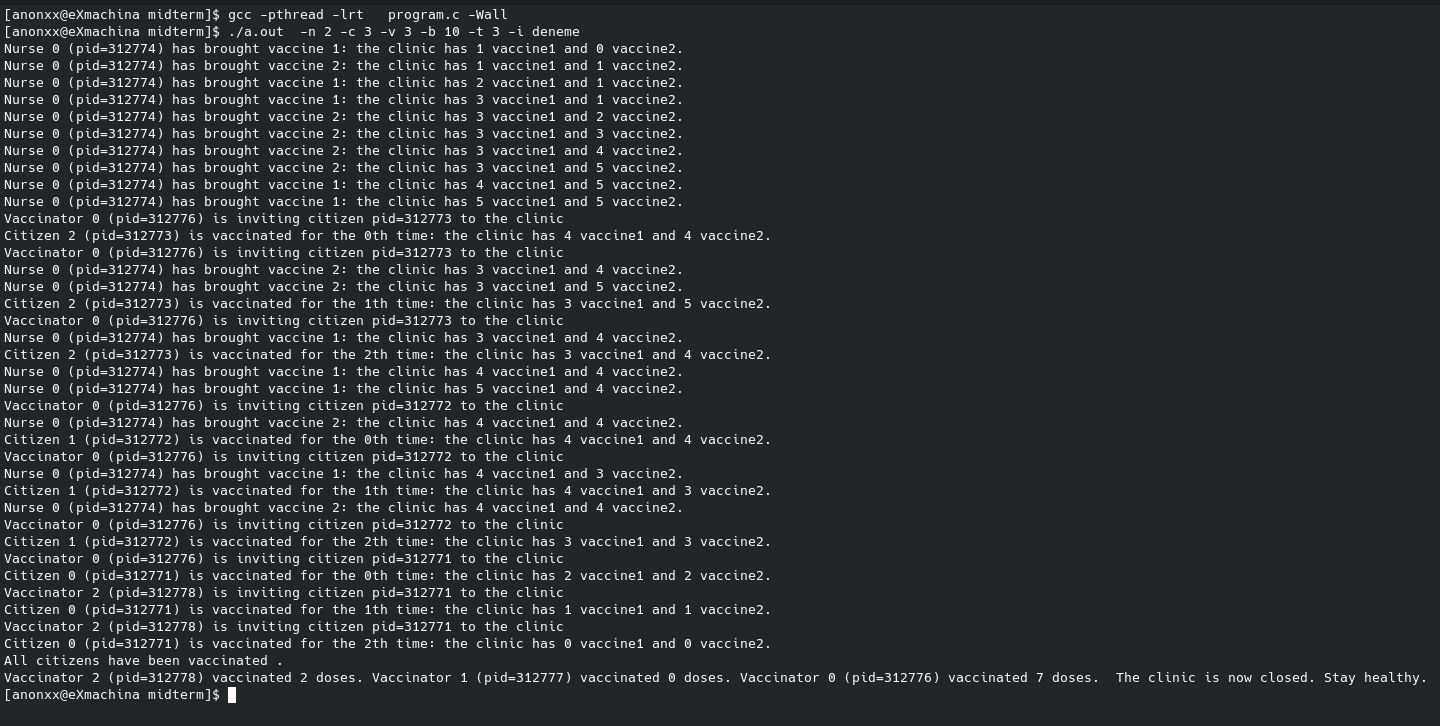
\includegraphics[width=\textwidth,height=\textheight,keepaspectratio]{images/output.png}

{\huge \textbf{The Requirements I have achieved} \\}
{\large For the bonus part as you see above I can vaccinate them in pid order but first it makes all doses for older citizen then it goes forward to next process ids }
 {\large I tried the rules below and they worked properly on my computer}
 
\begin{enumerate}
    \item {\large No compilation error }
    \item {\large No compilation warning}
    \item {\large \check{Makefile} }
    \item {\large \check{Report in Latex format}}
    \item {\large Printed usage information in case of missing or invalid argument}
    \item {\large Program did not crashed}
    \item {\large No memory leaks}
    \item {\large No zombie process}
    \item {\large No deadlock}
    \item {\large No poor synchronization}
    \item {\large Submitted on time}
    \item {\large Informed user in case of system errors}
    \item {\large If all processes get created, and at least one citizen is vaccinated at least once, yes.}
    
\end{enumerate}

{\huge \textbf{The Requirements I have failed} \\}

{\large I could not handled CTRL+C termination signal\\}


\end{document}
